\documentclass[11pt]{article}


\usepackage[margin=1in]{geometry}
\usepackage{amsmath,amssymb,amsthm}
\usepackage{graphicx}
\usepackage{booktabs}
\usepackage[hidelinks]{hyperref}
\renewcommand\labelitemi{$\bullet$}
\newtheorem{theorem}{Theorem}
\newtheorem{proposition}[theorem]{Proposition}
\newtheorem{corollary}[theorem]{Corollary}
\theoremstyle{definition}
\newtheorem{definition}[theorem]{Definition}
\newcommand{\grade}[1]{\textsf{\small[#1]}}
\newcommand{\Tr}{\operatorname{Tr}}
\newcommand{\Var}{\operatorname{Var}}
\newcommand{\F}[1]{\lVert #1\rVert_F}
\title{What the Present Must Keep:\\[2pt] the Weight Between, the Speed of the Record,\\ and the Wall It Survives}
\author{Jeromie Beasley}
\date{2 November 2026 \quad (version 1.1)}
\begin{document}
\maketitle

\noindent\emph{AI-assisted. The ideas and research direction are the author's; AI tools (Claude, Anthropic) were used for literature search, computation, drafting and typesetting. All simulations are runs of S.~McCormick's public code and of finite models on a cloud computer, not laboratory experiments.}

\begin{abstract}
A reduced description must carry, besides what it reads now, whatever the future still needs: that difference is memory. We put four finite results and one physical system in a single line. (i) In finite dimensions the first $\dim V$ readings decide every future reading, and a present reading needs no memory exactly when it closes under the evolution; under reduction the memory is the kernel $Be^{Du}C$ and its zero-lag trace is the coupling energy $E_B=\F{PH(1-P)}^2$, which is also the speed of the kept sector and the variance of its energy. (ii) Read at powers of the gap, the same weight is the projector metric ($k=-2$), the static optical response ($k=-1$), the energy variance ($k=0$) and the oscillator-strength budget ($k=+1$); log-convexity of these moments, a classical fact, makes the known bound $\alpha_0\le2(g^2F)^{1/3}$ a single ladder step, with equality when one gap value carries all the coupling. (iii) The log-odds $\tau=\log\det(I-C)-\log\det C$ of a cut obeys $\dot\tau^2\le4gS$ with $S=\Tr[(C(I-C))^{-1}]$, so a record moves no faster than $2\sqrt{E_BS}$. (iv) The projector is blind to an added constant; a clock reads only differences of constants; the operator's contour ledger reads the constant itself. (v) For idempotents the tangent form has neutral signature and can change sign. In an explicit chart the wall sits exactly on the line where the projector becomes orthogonal, the null direction there is a nilpotent push, and the contour ledger passes through unchanged in kind. A source inserted into the ledger rebuilds the wall when it is read in full; the geometry built from its real part alone is blind to the wall and keeps one trace of it, being positive semidefinite exactly on the wall. The physical case is neutrinos leaving a collapsing patch of the early universe. Their kept population obeys the one-mode form of the speed limit, which free streaming nearly saturates. Pre-registered runs of McCormick's code show that the history of decoupling, not only its end, sets the threshold for black-hole formation. A first-principles ledger built from the light that has already left carries about half of that memory; the rest sits in angular moments that no fluid closure keeps. Every claim is graded.
\end{abstract}

\paragraph{Grades.} \grade{T}: written proof here (Appendix~A). \grade{C}: cited result, restated. \grade{N}: computation reported with its script. \grade{M}: measured in a simulation run, with pre-registered kill lines. \grade{H}: interpretation. \grade{L}: finite statement checked in Lean at a named repository.

\section{The question}

Every description that keeps less than everything faces two questions. What must the present keep in order to predict every reading the future can still make? And what does it cost to move what is kept? This paper answers both in finite dimensions, joins the answers to a single quantity, the weight between a kept sector and the rest, and then tests the result on one physical system where the answer matters: neutrinos that stop scattering while a region of the early universe collapses.

The pieces were developed separately: the memory and weight results in \emph{The Weight Between}~\cite{WB}, the record's speed limit in \emph{The Offset Speed Limit}~\cite{OSL}, the transition-resolved optics in \emph{Light Keeps the Ledger}~\cite{LKL}, the sign wall in \emph{The Ledger Outlives the Metric}~\cite{GLO}, and the neutrino runs in \emph{When the Neutrinos Leave}~\cite{NL}. Here they are made one argument, every imported result is restated with its proof, and four links between them are new: the identification of the open fourth rung of the gap ladder (Section~\ref{sec:ladder}); the neutrino speed bound as the one-mode speed limit (Section~\ref{sec:speed}); the second reader of a constant (Section~\ref{sec:readers}); and the location and anatomy of the sign wall together with what a source can read there (Section~\ref{sec:wall}).

\section{Memory is what a reduction leaves out}\label{sec:memory}

Let $V$ be finite-dimensional, $L:V\to V$ the evolution and $R:V\to W$ the present reading. Write $N_\infty=\bigcap_{n\ge0}\ker RL^n$ for the differences that are never seen and $V_{\rm pred}=V/N_\infty$.

\begin{theorem}[the future is decided early]\label{thm:early}
$RL^nv=RL^nw$ for all $n$ if and only if it holds for $n<\dim V$. $N_\infty$ is $L$-invariant and lies in $\ker R$. \grade{T; L~\cite{WB}}
\end{theorem}

\begin{theorem}[least predictor]\label{thm:least}
If a linear $F$ determines every future reading, then $\ker F\subseteq N_\infty$ and $\operatorname{rank}F\ge\dim V_{\rm pred}$; $V_{\rm pred}$ with its induced dynamics is a predictor of least dimension. \grade{T; L}
\end{theorem}

\begin{theorem}[when the present closes]\label{thm:close}
The present reading needs no memory ($Rv=0\Rightarrow RLv=0$) if and only if $RL=AR$ for some linear $A$; then $N_\infty=\ker R$. Otherwise the present must carry $\dim V_{\rm pred}-\operatorname{rank}R>0$ further numbers. \grade{T; L}
\end{theorem}

Theorem~\ref{thm:early} is the finite observability statement of control theory~\cite{Kalman}; its use here is as the definition of memory: memory is the gap in Theorem~\ref{thm:close}.

\paragraph{Memory appears under reduction.} Split a Hermitian generator by an orthogonal projector $P$, $\dot x=-i(H_{PP}x+By)$, $\dot y=-i(B^\dagger x+H_{QQ}y)$ with $B=PH(1-P)$. Eliminating $y$,
\begin{equation}\label{eq:kernel}
\dot x(t)=-iH_{PP}x(t)-iBe^{-iH_{QQ}t}y(0)-\int_0^tK(t-s)\,x(s)\,ds,\qquad K(u)=Be^{-iH_{QQ}u}B^\dagger .
\end{equation}
The convolution is the memory and the middle term is the hidden preparation~\cite{Zwanzig}. The memory vanishes at every lag exactly when $B=0$, and its zero-lag trace is
\begin{equation}\label{eq:EB}
\Tr K(0)=\F{B}^2=E_B ,
\end{equation}
the \emph{weight between} $P$ and $1-P$ \grade{T}.

\section{The weight between}\label{sec:weight}

\begin{proposition}[every motion of what is kept is a crossing]\label{prop:offdiag}
If $P^2=P$ and $V=PV+VP$, then $PVP=0=(1-P)V(1-P)$ and $V=PV(1-P)+(1-P)VP$. \grade{T; L~\cite{GLO,LKL}}
\end{proposition}

This holds for every idempotent, orthogonal or not. For orthogonal $P$ moving under $\dot P=-i[H,P]$,
\begin{equation}\label{eq:gEB}
g:=\tfrac12\F{\dot P}^2=\tfrac12\F{[H,P]}^2=E_B,\qquad\text{and }g=\Var_\psi H\text{ when }P=|\psi\rangle\langle\psi| ,
\end{equation}
so one number is at once the speed of the kept sector, the zero-lag memory \eqref{eq:EB} and, for a pure state, the energy variance (Anandan--Aharonov~\cite{AA}) \grade{T; N: worst relative difference $4\times10^{-15}$ over 300 cases~\cite{WB}}. On the tangent space of orthogonal projectors $Q(V,W)=\Tr(PVW)$ is positive semidefinite; its real part is the metric $g$ and $\Omega=2\operatorname{Im}Q$ is the curvature, so $4\det g\ge\Omega^2$ and zero metric forces zero curvature \grade{T}.

\subsection{The gap ladder}\label{sec:ladder}

Fix Hermitian couplings $K_{ij}=\overline{K_{ji}}$ between levels $d_i$ with gaps $\Delta_{ij}=d_i-d_j\ne0$ wherever $K_{ij}\ne0$, and set $S_k=\sum_{i\ne j}|K_{ij}|^2|\Delta_{ij}|^k$.

\begin{proposition}[log-convex ladder]\label{prop:ladder}
$k\mapsto\log S_k$ is convex; in particular $S_k^2\le S_{k-j}S_{k+j}$ and, for $a<b<c$, $S_b^{\,c-a}\le S_a^{\,c-b}S_c^{\,b-a}$. \grade{C: Hardy--Littlewood--P\'olya~\cite{HLP}; T; L for the middle rung $S_0^2\le S_{-2}S_2$}
\end{proposition}

On the ground row the same construction gives $S^{(0)}_k=\sum_{n\ne0}|K_{n0}|^2\Delta_n^k$, with $\Delta_n=d_n-d_0>0$ and $K$ a perturbation of the ground level; it is log-convex by the same argument. Writing $S_k$ for $S^{(0)}_k$ below, the rungs are

\begin{center}\begin{tabular}{cll}\toprule
$k$ & ground-row moment & reading\\\midrule
$-2$ & $S_{-2}=\sum_n|K_{n0}|^2/\Delta_n^2=g_{KK}$ & fidelity (projector) metric: memory geometry\\
$-1$ & $2S_{-1}=\alpha_0$ & static response to the probe $K$: light\\
$0$ & $S_0=\Var_0K$ & energy variance: the speed of time, \eqref{eq:gEB}\\
$+1$ & $S_{+1}=\tfrac12\langle0|[K,[H,K]]|0\rangle=F$ & oscillator-strength budget\\\bottomrule
\end{tabular}\end{center}

The last row is new to the ladder of~\cite{WB}, where rung $+1$ was left open.

\begin{proposition}[rung $+1$ is the oscillator budget]\label{prop:rung1}
For $H=\operatorname{diag}(d)$ with $d_0$ the lowest level, $\tfrac12\langle0|[K,[H,K]]|0\rangle=\sum_n\Delta_n|K_{n0}|^2$. For $K=qx$ and $H=p^2/2m+V(x)$ this is the Thomas--Reiche--Kuhn sum $q^2\hbar^2/2m$. \grade{T; C~\cite{BL}; N: worst relative error $1.2\times10^{-14}$ over 2000 random cases}
\end{proposition}

\begin{corollary}[the optical bound is a ladder step]\label{cor:alpha}
$\alpha_0\le2\,(g_{KK}^2F)^{1/3}$, with equality if and only if all the coupling sits at a single gap value. \grade{T; N: no violation in 2000 random spectra, equality for one gap to $4\times10^{-16}$}
\end{corollary}

This bound was proved in~\cite[Cor.~4.8]{LKL} by H\"older's inequality on the spectral measure; Proposition~\ref{prop:ladder} with $(a,b,c)=(-2,-1,1)$ shows it is one step of the ladder, and Proposition~\ref{prop:rung1} identifies its third quantity as rung $+1$. The confined oscillator of~\cite[Sec.~4.10a]{LKL} has a single dipole-active gap and saturates it (Figure~\ref{fig:ladder}). Inequalities between neighbouring moments of optical absorption, including the Cauchy--Schwarz step $S_{-1}\le\sqrt{S_0S_{-2}}$, are known in the quantum-geometry literature~\cite{SWM,OF,Pant}; what is added here is the reading of the four rungs as one weight and the identification of the open rung.

\begin{figure}[t]\centering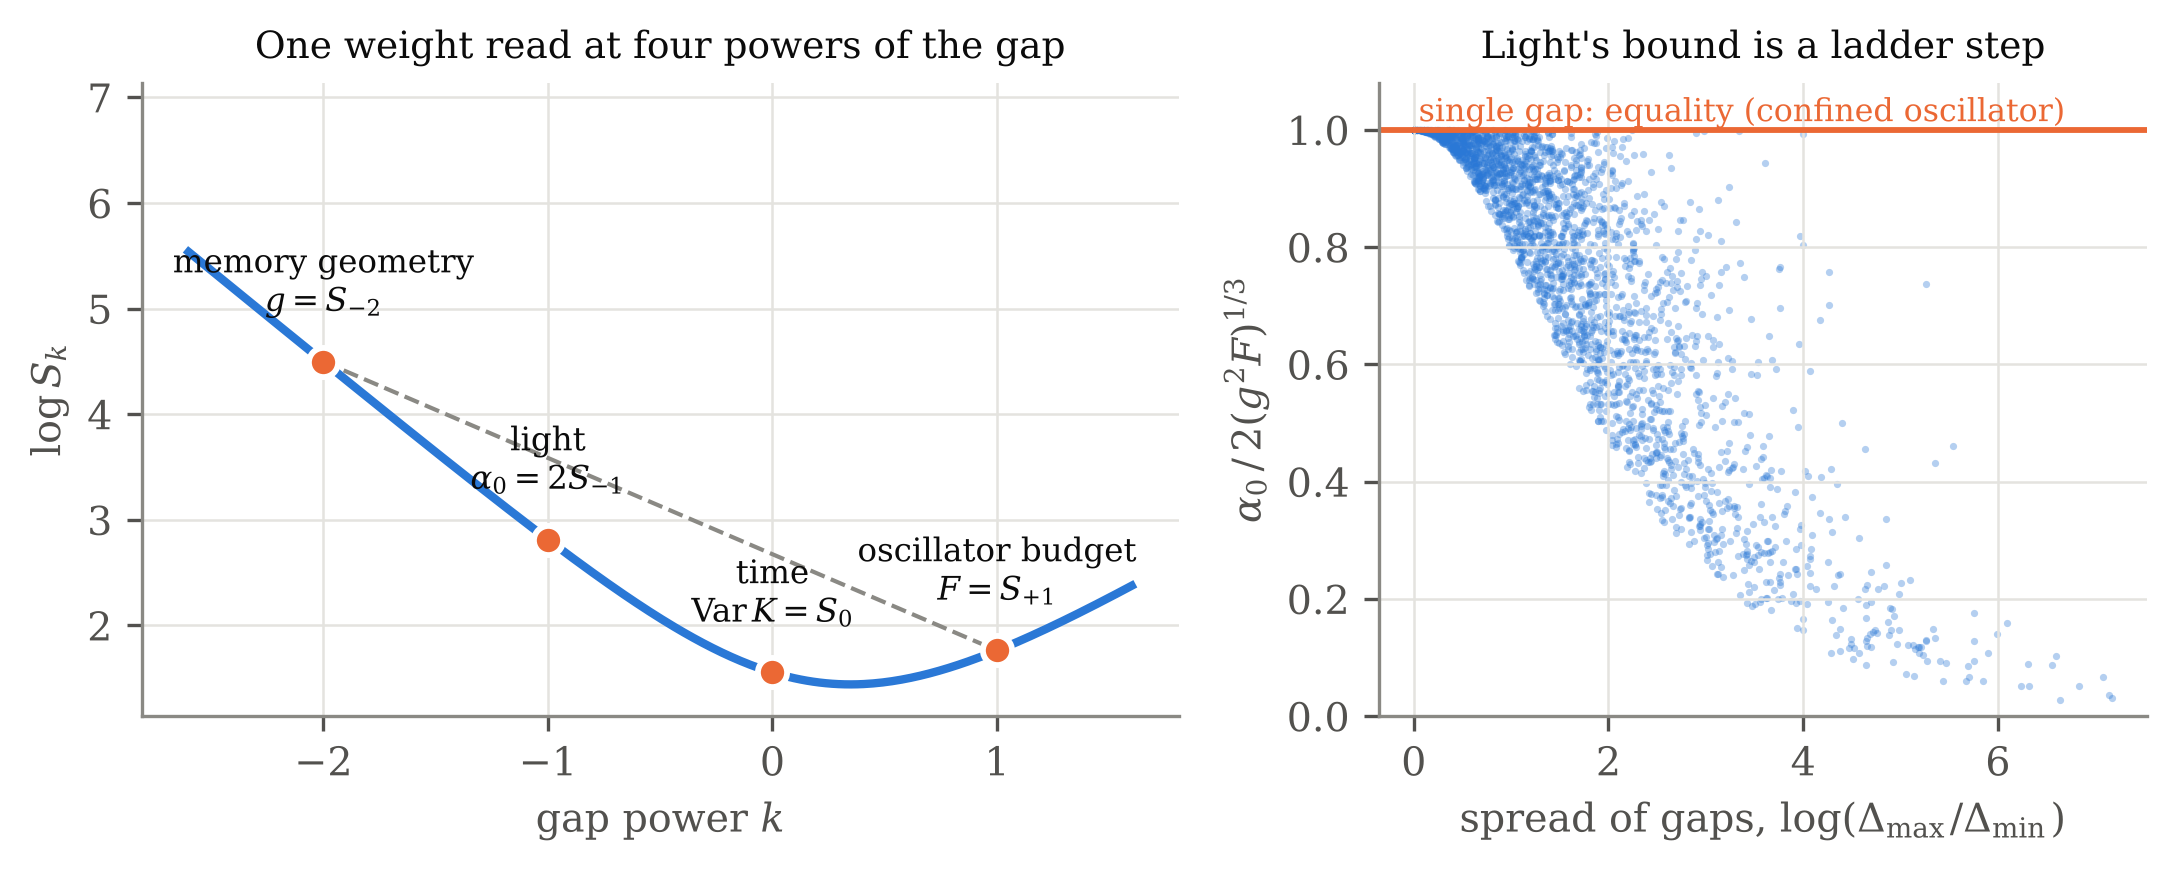
\includegraphics[width=\textwidth]{figs/jfig1_ladder.png}
\caption{Left: the ground-row ladder $\log S_k$ for a random seven-level coupling. Its four integer rungs are the memory geometry, the static optical response, the energy variance and the oscillator budget; the curve is convex. The dashed chord from $k=-2$ to $k=+1$ lies above rung $-1$: that gap is the inequality $\alpha_0\le2(g^2F)^{1/3}$. Right: the ratio $\alpha_0/2(g^2F)^{1/3}$ over 3000 random spectra against the spread of their gaps. It never exceeds one and reaches one only when a single gap carries the coupling, as in the confined oscillator.}\label{fig:ladder}\end{figure}

\section{The record and its speed limit}\label{sec:speed}

Cut an orthogonal projector $P$ on $\mathbb C^n$ by a fixed isometry $E:\mathbb C^m\to\mathbb C^n$ into the accessible block $C=E^\dagger PE$, with $0<C<I$. Then $C-C^2=P_{12}P_{12}^\dagger$ \grade{T; L~\cite{LKL}}, the census of the cut. The \emph{offset}
\begin{equation}\label{eq:offset}
\tau=\Tr[\log(I-C)-\log C]=\log\det(I-C)-\log\det C
\end{equation}
is the log-odds of the block being empty against full~\cite{OBB}. The census loses its sign: $C=\operatorname{diag}(0.2,0.8)$ and $\operatorname{diag}(0.2,0.2)$ have the same census and offsets $0$ and $\log16$.

\begin{theorem}[the offset speed limit]\label{thm:osl}
For a differentiable family of orthogonal projectors, with $g=\tfrac12\F{\dot P}^2$ and $S=\Tr[(C(I-C))^{-1}]$,
\begin{equation}\label{eq:osl}
\dot\tau^2\le4gS .
\end{equation}
Equality holds if and only if $\dot P=\lambda[P,[P,F]]$ for real $\lambda$, where $F=EWE^\dagger$, $W=-(C(I-C))^{-1}$. \grade{T; for rank one a bound of Mandelstam--Tamm type~\cite{MT}; N: largest ratio $0.911$ over 500 driven cases, equality case to $7\times10^{-9}$~\cite{OSL}}
\end{theorem}

\begin{corollary}[a record moves only as fast as the weight between]\label{cor:record}
If $\dot P=-i[H,P]$, then $|\dot\tau|\le2\sqrt{E_BS}$. If $PH(1-P)=0$ the offset is frozen. \grade{T}
\end{corollary}

\paragraph{One accessible mode.} For $m=1$ and a pure state, $C=A$ is the population kept in the accessible mode, $\tau=\log[(1-A)/A]$, $\dot\tau=-\dot A/(A(1-A))$, $S=1/(A(1-A))$, and \eqref{eq:osl} becomes
\begin{equation}\label{eq:onemode}
\dot A^2\le4\,g\,A(1-A),\qquad g=\Var_\psi H .
\end{equation}
Under unitary evolution $\Var_\psi H$ is conserved, so $g$ is its value at the start \grade{T}. For an orthogonal rank-one projector path in $\mathbb C^2$ the gap is exact: $4gS-\dot\tau^2=4(\operatorname{Im}\bar b\dot b)^2/(c(1-c))^2$ for $P=\begin{pmatrix}c&b\\\bar b&1-c\end{pmatrix}$ \grade{T; L; N~\cite{OSL}}. Equation~\eqref{eq:onemode} is exactly the speed bound found for neutrinos in~\cite{NL}; Section~\ref{sec:nu} uses it.

\section{Two readers of a constant}\label{sec:readers}

\begin{proposition}[what sees $sH+cI$]\label{prop:readers}
Let $s>0$ and $c\in\mathbb R$.
(a) The spectral projectors of $H$, and the tensor $Q$ of Section~\ref{sec:weight}, are unchanged by $H\mapsto sH+cI$.
(b) Every expectation value in a single branch is unchanged by $H\mapsto H+cI$; two branches with constants $c_1,c_2$ acquire the relative phase $-(c_1-c_2)t$.
(c) For a positive operator $K$ and a contour $\Gamma$ enclosing a selected cluster of $k$ eigenvalues $\lambda_j$ and kept away from the negative axis, the contour ledger $Z_\Gamma(K)=\frac1{2\pi i}\oint_\Gamma\log z\,\Tr(z-K)^{-1}dz$ obeys, for $\alpha>0$ and every $c$ with $\lambda_j+c>0$ and the shifted contour still separating the cluster,
\begin{equation}\label{eq:Zshift}
Z_{\Gamma+c}(K+cI)=Z_\Gamma(K)+\sum_j\log(1+c/\lambda_j),\qquad Z_{\alpha\Gamma}(\alpha K)=Z_\Gamma(K)+k\log\alpha ,
\end{equation}
while the projector does not move. \grade{T; L for (a) and (b)~\cite{OSL}; (c) C~\cite[Prop.~30]{GLO}; N: (c) to every printed digit, projector change $<10^{-15}$; L for the eigenvalue identity in (c)}
\end{proposition}

So the geometry of the kept subspace sees neither seconds nor a constant. Among readings of a state, only a comparison of two clocks sees a constant, and then only as a difference: this is how gravity first appeared in a neutron interferometer~\cite{COW} and how satellite clocks are corrected. The operator's own contour ledger reads the constant directly. The ledger and the clock are therefore the two readers of a weight, and the projector is the reader of a direction \grade{H}. The proposal of~\cite{OSL} that a pair of clocks of different kinds can test whether every form of energy carries the same weight (a strontium optical clock against a thorium-229 nuclear clock, whose ratio cancels the universal part exactly) is the experimental form of reading (b) \grade{N: one year of the ratio resolves a coupling to $7.6\times10^{-11}$ in a model with stated inputs; H}.

\section{The wall the record survives}\label{sec:wall}

\subsection{Two kinds of wall}

For an orthogonal projector the tangent pairing is a Gram form, $Q(V,V)=\F{(1-P)VP}^2\ge0$: the metric can lose rank but never sign~\cite{LKL}. For an idempotent that is not orthogonal it can do both.

\begin{theorem}[neutral signature]\label{thm:neutral}
On the full real tangent space of rank-$k$ idempotents in $M_n(\mathbb C)$, $q(D)=\tfrac12\operatorname{Re}\Tr D^2$ is nondegenerate with signature $(2k(n-k),2k(n-k))$. \grade{T; L for the coordinate algebra~\cite{GLO}; N: confirmed for five $(n,k)$ from the null space of $D\mapsto PD+DP-D$; the Hermitian slice is positive definite}
\end{theorem}

\begin{theorem}[a negative direction lifts the overlap above the cap]\label{thm:cap}
For a $C^2$ family of rank-$k$ idempotents with $D=P'(0)$, $\operatorname{Re}\Tr(P(0)P(t))=k-\tfrac12\operatorname{Re}\Tr(D^2)\,t^2+o(t^2)$. If $q(D)<0$ the overlap exceeds $k$ for all small $t\ne0$. \grade{T; L~\cite{GLO}; N: 40-digit check, relative error $3.5\times10^{-6}$}
\end{theorem}

For orthogonal projectors $\Tr(PR)\le k$ always; the cap is a property of the orthogonal class, and losing it is what a sign wall means.

\subsection{An explicit wall, and where it sits}

On $|x|,|y|<\tfrac14$ put $z=x+iy$, $w=x+iy^2$ and
\begin{equation}\label{eq:chart}
P(x,y)=\frac1{1+zw}\begin{pmatrix}1&w\\z&zw\end{pmatrix},\qquad H=(2+\tfrac y{10})P+(5+\tfrac y5)(I-P).
\end{equation}

\begin{theorem}[a wall without an exceptional point]\label{thm:chart}
$P^2=P$, $\Tr P=1$, and on $x=0$ the form $g_{ij}=\tfrac12\operatorname{Re}\Tr(\partial_iP\,\partial_jP)$ is $(1-y^3)^{-2}\operatorname{diag}(1,-2y)$: positive definite for $y<0$, indefinite for $y>0$. The eigenvalues of $H$ stay separated by $3+y/10$; the circle $|z-2|=0.4$ encloses one of them, giving count $N=1$ and ledger $Z=\log(2+y/10)$, regular and varying through the wall. \grade{C~\cite{GLO}; T (A.8); N: exact symbolic check and contour quadrature to $3\times10^{-16}$}
\end{theorem}

The new statement is where the wall is and what its null direction is.

\begin{proposition}[the wall is the edge of the self-adjoint slice]\label{prop:edge}
In the box of \eqref{eq:chart}:
(i) $P(x,y)$ is self-adjoint if and only if $y=0$.
(ii) On $y=0$, $g=(1+x^2)^{-2}\operatorname{diag}(1,0)$, so $\det g=0$ along the whole line, and $\det g$ changes sign across it.
(iii) $\partial_zP$ is nilpotent everywhere; on $y=0$, $\partial_yP=i\,\partial_zP$ is a nonzero, non-self-adjoint nilpotent, so $\tfrac12\operatorname{Re}\Tr(\partial_yP)^2=0$ while $\tfrac12\F{\partial_yP}^2>0$.
\grade{T (A.8); L for (i) and the nilpotent square in (iii); N: symbolic check, and on a $401\times401$ grid the zero set of $\det g$ is $y=0$ for every $x$}
\end{proposition}

So the metric goes null exactly where the projector is most ordinary, and the direction it cannot price is a push off the orthogonal projectors that squares to zero. The example after Theorem~2 of~\cite{GLO}, a self-adjoint point carrying a negative tangent, and the wall of Theorem~\ref{thm:chart} are one phenomenon. Part~(iii) also shows that the weight $\tfrac12\F{\dot P}^2$ of Section~\ref{sec:weight} stays positive through the wall: it cannot see it. Whether the wall sits on the self-adjoint locus in every analytic chart is untested.

\begin{figure}[t]\centering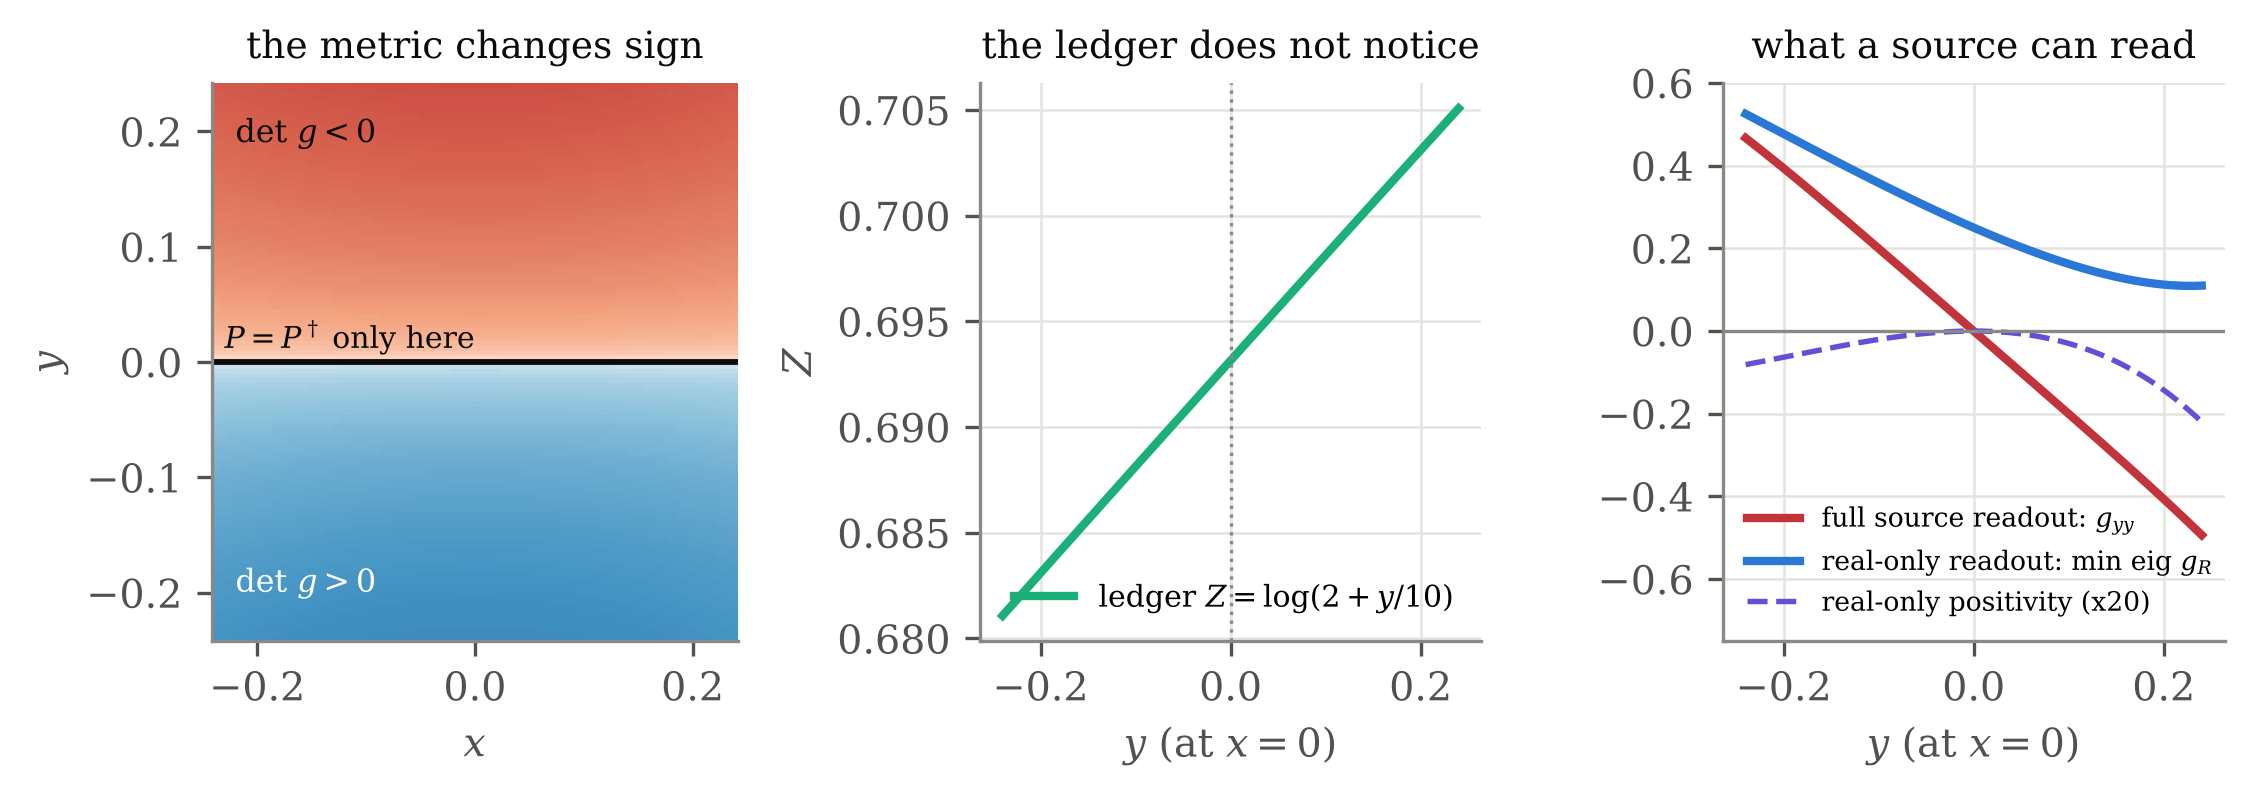
\includegraphics[width=\textwidth]{figs/jfig2_wall.png}
\caption{The sign wall of \eqref{eq:chart}. Left: the sign of $\det g$ over the box (fourth root of its size for contrast). The black line $y=0$ is both the wall and the only place where $P=P^\dagger$. Centre: the contour ledger $Z=\log(2+y/10)$ crosses the wall without a feature. Right: what a source inserted into the ledger can read along $x=0$. Read in full (real and imaginary parts), it rebuilds $g_{yy}$, which changes sign at the wall. Read through its real part only, it rebuilds a geometry whose smallest eigenvalue stays positive, blind to the wall; its own positivity (dashed, scaled by 20) is negative off the wall and touches zero exactly on it.}\label{fig:wall}\end{figure}

\subsection{What a source can read}

The bare ledger $Z$ cannot see the projector at all: with $H=\lambda P+\mu(1-P)$, $Z=k\log\lambda$ depends only on $\lambda$, while $g$ depends only on $P$ \grade{T~\cite{GLO}}. A probe restores the link.

\begin{theorem}[source insertion]\label{thm:source}
For invertible $K$, a contour $\Gamma$ separating a cluster with an analytic logarithm, and a fixed $B$,
\begin{equation}\label{eq:source}
\frac{d}{dt}Z_\Gamma(K+tB)\Big|_0=\Tr(P_\Gamma K^{-1}B),
\end{equation}
including clusters with Jordan blocks. Write $q(b)$ for \eqref{eq:source} with the probe $B=bb^\dagger$. For any such $K$ the complex readings at $e_i$, $e_i+e_j$, $e_i+ie_j$ recover $P_\Gamma K^{-1}$ by polarisation. If $K=K^\dagger>0$, then $q(b)=b^\dagger P_\Gamma K^{-1}b=\sum_{\lambda\in\Gamma}\lambda^{-1}\lVert P_\lambda b\rVert^2\ge0$, its null space is $\ker P_\Gamma$, and the recovered $P_\Gamma K^{-1}$ has support $P_\Gamma$. \grade{T; C~\cite{GLO,LKL}; N: finite differences of $Z$ against \eqref{eq:source}, worst relative error $7\times10^{-10}$ with Jordan clusters; tomography from measured derivatives to $6\times10^{-11}$}
\end{theorem}

For an oblique projector the response need not be positive: with $K=\begin{pmatrix}2&9\\0&5\end{pmatrix}$, $P_\Gamma=\begin{pmatrix}1&-3\\0&0\end{pmatrix}$ and $b=(1,1)$, $q(b)=-1$ although both eigenvalues are positive \grade{T~\cite{GLO}; N}. Light's probe-span result~\cite[Sec.~4.9b]{LKL} already states that full response needs probes resolving the imaginary cross components. At the wall this becomes sharp.

\begin{proposition}[full and real-only readout at the wall]\label{prop:readout}
For the chart \eqref{eq:chart}, with every $q(b)$ measured as a finite difference of the contour ledger:
(a) the full readout, polarising with complex probes, rebuilds $P$ to $9\times10^{-10}$ and the metric to $8\times10^{-6}$, and places the wall at $y=-3.8\times10^{-7}$;
(b) the real-only readout, $\operatorname{Re}q$, recovers only the self-adjoint part of $P_\Gamma K^{-1}$; the geometry built from it is positive definite throughout, smallest eigenvalue $0.093$ on a $41\times41$ grid over $|x|,|y|\le0.24$;
(c) the smallest eigenvalue of $\tfrac12(P+P^\dagger)/\lambda$ is negative everywhere off $y=0$ (down to $-0.011$) and exactly zero on all 41 grid points of $y=0$;
(d) for an orthogonal-projector family the real-only readout equals the full readout to $1.3\times10^{-11}$ and there is no wall.
\grade{N: kill lines written before the run, all met}
\end{proposition}

The metric a source rebuilds therefore shows the sign wall when the source is read with its phase, and does not when only its real part is read. Part (b) is generic: the self-adjoint parts of independent tangents always give a positive form, so the real readout cannot locate the wall. It keeps one trace of it, part (c): its own response is positive semidefinite exactly on the wall and indefinite everywhere else in the box \grade{N; H}.

\section{The physical case: neutrinos leaving a collapsing patch}\label{sec:nu}

Primordial black holes heavier than about $10^6M_\odot$ form while neutrinos, 41\% of the radiation, stop scattering. McCormick evolved them with their angle-resolved transport equation in spherical general relativity and found that free streaming raises the collapse threshold, by $\Delta C_{l,c}/C_{l,c}\simeq0.235R_\nu$; under gradual decoupling, $\kappa=H(\epsilon_{\rm dec}/\epsilon)^3$, only a share $G=(\delta_c-\delta_c^{\rm fluid})/(\delta_c^{\rm inst}-\delta_c^{\rm fluid})$ survives~\cite{McC}. Here $\epsilon=1/(aHr_m)$; in his initial data the conformal time in units of $r_m$ equals $\epsilon$, so $\epsilon$ is the time variable below \grade{T}.

\subsection{The cut and the weight}

One Fourier mode of the linearised intensity evolves under $\partial_\epsilon v=-(ikM+\sigma(\epsilon)(I-P_0))v$ in the normalised Legendre basis, with $M$ real symmetric tridiagonal, $M_{\ell,\ell+1}=M_{\ell+1,\ell}=c_\ell=(\ell+1)/\sqrt{(2\ell+1)(2\ell+3)}$, $P_0=|0\rangle\langle0|$ and $\sigma=\epsilon_{\rm dec}^n/\epsilon^{n+1}$. Collisions conserve the isotropic part and remove the rest. The kept sector is $|0\rangle$, the density, and the weight between it and everything that streams is
\begin{equation}
E_B=\F{P_0\,kM\,(1-P_0)}^2=k^2c_0^2=k^2/3,
\end{equation}
so $\sqrt{E_B}=k/\sqrt3$ is the radiation sound speed \grade{T}. All non-normality of the single-rate operator lies on the density--flux link, $\tfrac18\F{[L,L^\ast]}^2=\kappa^2k^2/3$ \grade{T~\cite{NL,CE}}. Collisions act on the hidden moments only, so the kept population changes only through that link: light writes the kept sector's record and collisions only erase what is hidden \grade{T}.

\paragraph{The memory kernel.} In the relaxation model every hidden moment is damped at the same rate, so the hidden propagator is exact, $U_Q(t,r)=e^{-[\Sigma(t)-\Sigma(r)]}e^{-ik(t-r)M_{QQ}}$ with $\Sigma=-\epsilon_{\rm dec}^n/(n\epsilon^n)$, and eliminating the hidden block gives
\begin{equation}\label{eq:nukernel}
\dot a(t)=S(t)-k^2c_0^2\int_s^t[U_Q(t,r)]_{11}\,a(r)\,dr ,
\end{equation}
which is \eqref{eq:kernel} with $B=kc_0\langle1|$, collisions entering as a time-dependent damping of the hidden block \grade{T}.

\paragraph{The speed limit.} With $A=|a_0|^2$, the one-mode limit \eqref{eq:onemode} with $g=E_B$ is
\begin{equation}\label{eq:nuspeed}
\dot A^2\le4E_B\,A(1-A),
\end{equation}
proved directly in~\cite{NL} with collisions included, since they only shorten the state \grade{T; L~\cite{NL}}. For pure streaming it is Corollary~\ref{cor:record} with $\Var_{|0\rangle}(kM)=k^2/3$ conserved (drift $2\times10^{-14}$), and the bound is met almost exactly: largest ratio $0.99996$ \grade{N}. Gradual decoupling holds the record back (Figure~\ref{fig:speed}).

\begin{figure}[t]\centering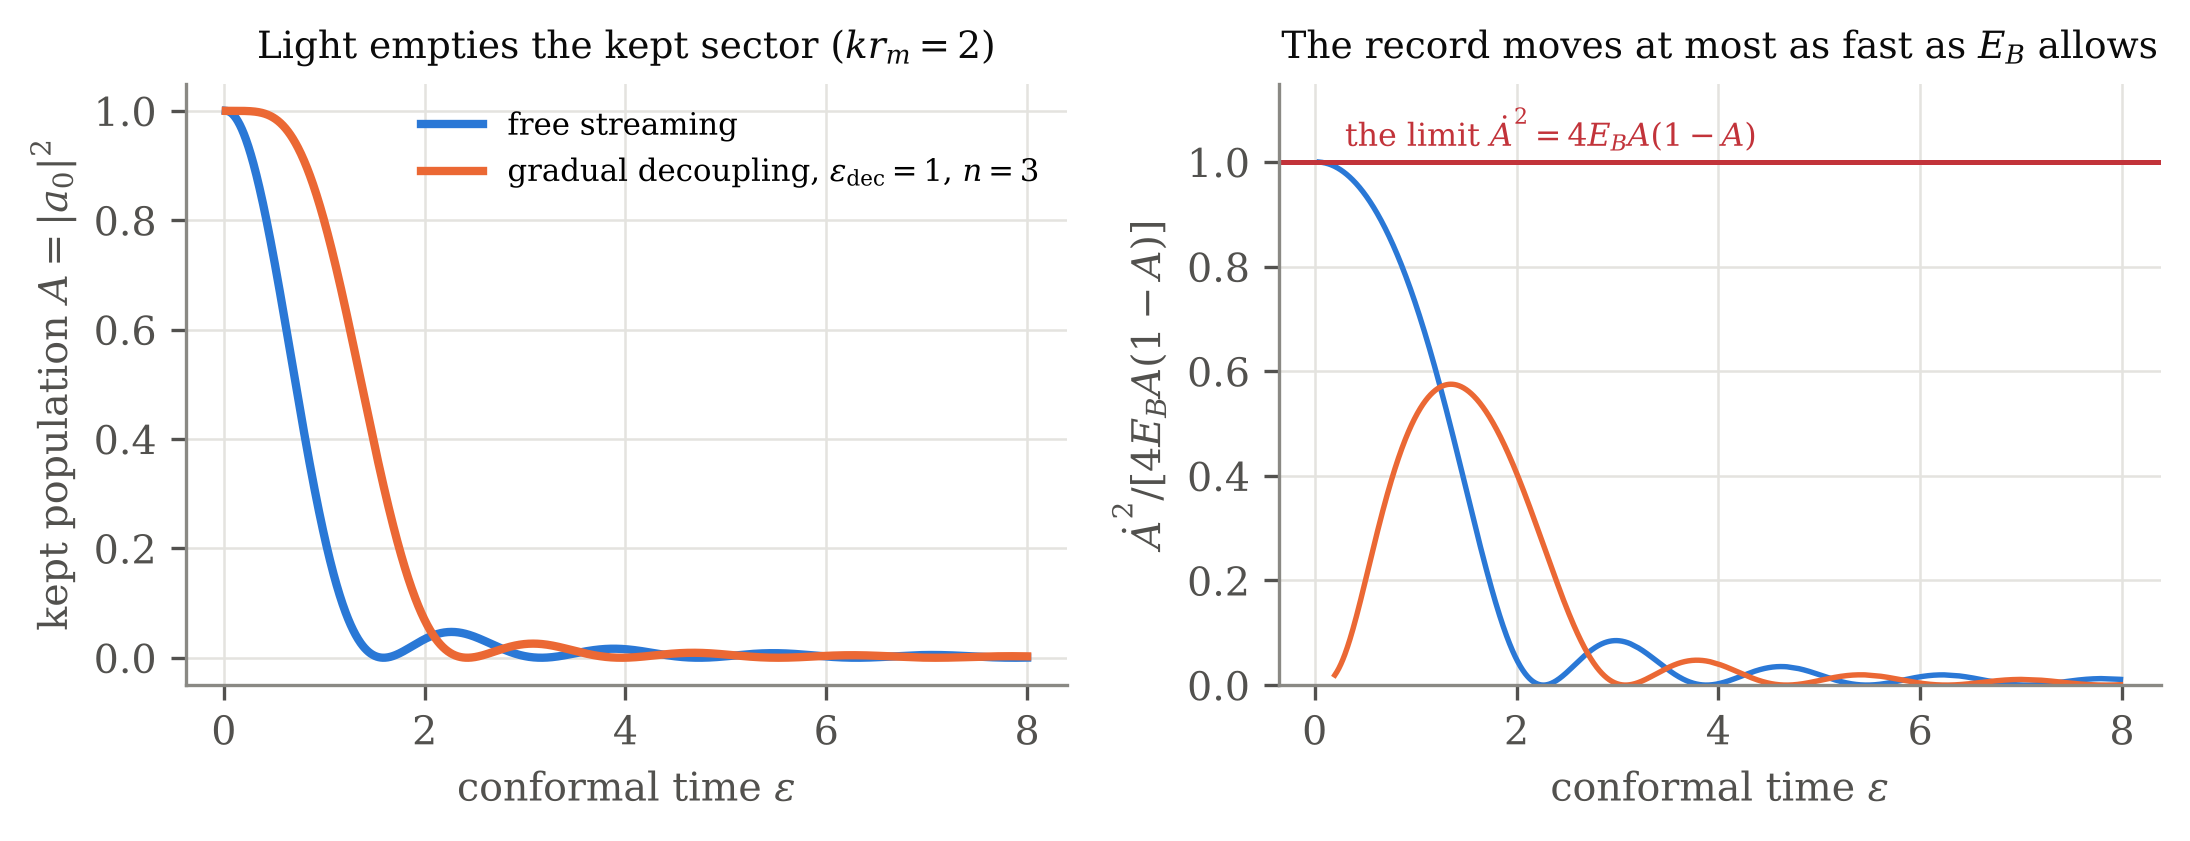
\includegraphics[width=\textwidth]{figs/jfig3_speed.png}
\caption{The record's speed limit on the neutrino kept mode, $kr_m=2$. Left: the population kept in the density moment. Right: $\dot A^2/[4E_BA(1-A)]$. Free streaming starts on the limit; gradual decoupling ($\epsilon_{\rm dec}=1$, $n=3$) reaches at most $0.58$ for this mode. Profile-averaged trajectories in~\cite{NL} reach $0.87$.}\label{fig:speed}\end{figure}

\subsection{The history is remembered}

McCormick's code~\cite{McCcode} was run unchanged except for the decoupling law, with every prediction and kill line written before the runs (Appendix~B). With $\kappa/H=(\epsilon_{\rm dec}/\epsilon)^6$, a steeper history, the surviving share is \grade{M}

\begin{center}\begin{tabular}{lccc}\toprule
& $\delta_c$ & $G$ ($n=6$) & $G$ ($n=3$)\\\midrule
C: $\epsilon_{\rm dec}=1$ & $0.51756\pm0.00019$ & $0.648\pm0.006$ & $0.683$\\
B: $\epsilon_{\rm dec}=2$ & $0.50743\pm0.00011$ & $0.317\pm0.004$ & $0.431$\\
D: $\epsilon_{\rm dec}=3$ & $0.50245\pm0.00019$ & $0.154\pm0.006$ & $\approx0.30$\\\bottomrule
\end{tabular}\end{center}

\noindent The $n=3$ column is McCormick's Table~II~\cite{McC}; at $\epsilon_{\rm dec}=3$, which he did not run, it is interpolated between his $0.431$ and $0.190$.

A population that decouples more abruptly by the same nominal time keeps less of its effect: a history-blind rule, which would give the interpolated $n=3$ value, misses Test D by $0.146$ against a kill line of $0.08$. Test B is unchanged by a tenfold higher rate cap ($-0.00003$) and by a finer grid ($+0.00008$). A broad profile that collapses twice as late keeps the same share or less ($G=0.181$, $0.045$ against $0.190$, $0.063$), so the collapse time alone does not set the clock \grade{M}. A memory form built on the kept sector, with one weight fitted to McCormick's curve and frozen, predicted Tests C, B, D as $0.663$, $0.246$, $0.118$ before they were run, all inside the kill line \grade{M; fit}.

\subsection{Where the memory sits}\label{sec:where}

Two neutrino states with the same density, flux and anisotropic stress, differing only in the $\ell=3$ or $\ell=4$ moment, were evolved under the same history with the difference planted at time $\epsilon_s$. Planted at or after decoupling, the difference returns into density, flux and stress at the level of 2--13\% (8--10\% read at $\epsilon=4$); planted deep in the coupled era it is erased by $\exp[-\epsilon_{\rm dec}^n/(n\epsilon_s^n)]$, down to $10^{-30}$. Every on/off call was written before the run and all came out as predicted; solving \eqref{eq:nukernel} from the closed-form $U_Q$ alone reproduces the full system to between $5\times10^{-8}$ and $7\times10^{-7}$ \grade{N~\cite{NL}}. In the language of Theorem~\ref{thm:close}: density, flux and stress do not close under the decoupling evolution, and the angular moments a fluid closure drops are among the numbers the present must carry.

\subsection{How much of the memory is in the ledger}

The last test asks the question of Section~\ref{sec:speed} directly: is the record written by light into the kept sector the whole memory? The kinetic model fixes the ledger with nothing fitted: $S(\epsilon)=\sum_kw_k|a_0(k,\epsilon)|^2$ with the profile weights $w_k\propto k^2e^{-k^2/2}$, and the entry written at time $\epsilon$ is $L(\epsilon)=-dS/d\epsilon$. If the threshold reads the ledger linearly, $\Delta\delta_c=\int W(\epsilon)L(\epsilon)\,d\epsilon$ with a listening weight $W$, then
\begin{equation}
G=\frac{\int W\,L_{\rm hist}}{\int W\,L_{\rm inst}}
\end{equation}
with no free parameter once $W$ is measured. $W$ was measured by short bursts of free streaming, $\kappa=0$ on $[\epsilon_b,1.25\epsilon_b]$, inside a fully coupled history, eight burst times, full threshold searches. Five kill lines were written before the runs \grade{M}:

\begin{center}\begin{tabular}{lll}\toprule
line & test & outcome\\\midrule
K1 & two bursts add & pass: $0.001333=0.000889+0.000444$\\
K2 & nine predicted $G$ within $0.05$ & \textbf{fail}: worst miss $0.101$ (Test C)\\
K3 & a coupling burst has the opposite sign & pass: $-0.00904$, $-0.00194$\\
K4 & quick readout within 20\% of full search & pass: within 15\%\\
K5 & equal ledgers give equal $G$ & pass, one pair: $0.686$ and $0.679$\\\bottomrule
\end{tabular}\end{center}

The listening weight falls from $0.028$ per ledger entry at $\epsilon_b=0.25$ to zero by $\epsilon_b=6$ (Figure~\ref{fig:ledger}). The shape of $G$ is right late and too low early, and the size is about half: the ledger reading of the instantaneous shift is $0.0157$ against the measured $0.0306$, short by a factor $1.9$--$2.3$ for every history. Measuring $W$ the opposite way, from coupling bursts on a free-streaming base, fails worse \grade{M}.

The reading is Theorem~\ref{thm:close} measured. The kept population is a present reading that does not close: late collisions stop neutrinos that are already in the hidden moments, on their way out, and hand their momentum back to the plasma. That moves the threshold strongly while barely changing the ledger. So the record of when the neutrinos left is written by light, and the ledger of light that has left holds about half of it; the other half is carried by light still in transit, in exactly the moments Section~\ref{sec:where} found holding the memory \grade{M; H}. A ledger that also books the hidden-moment flux is the natural next object; it is untested.

\begin{figure}[t]\centering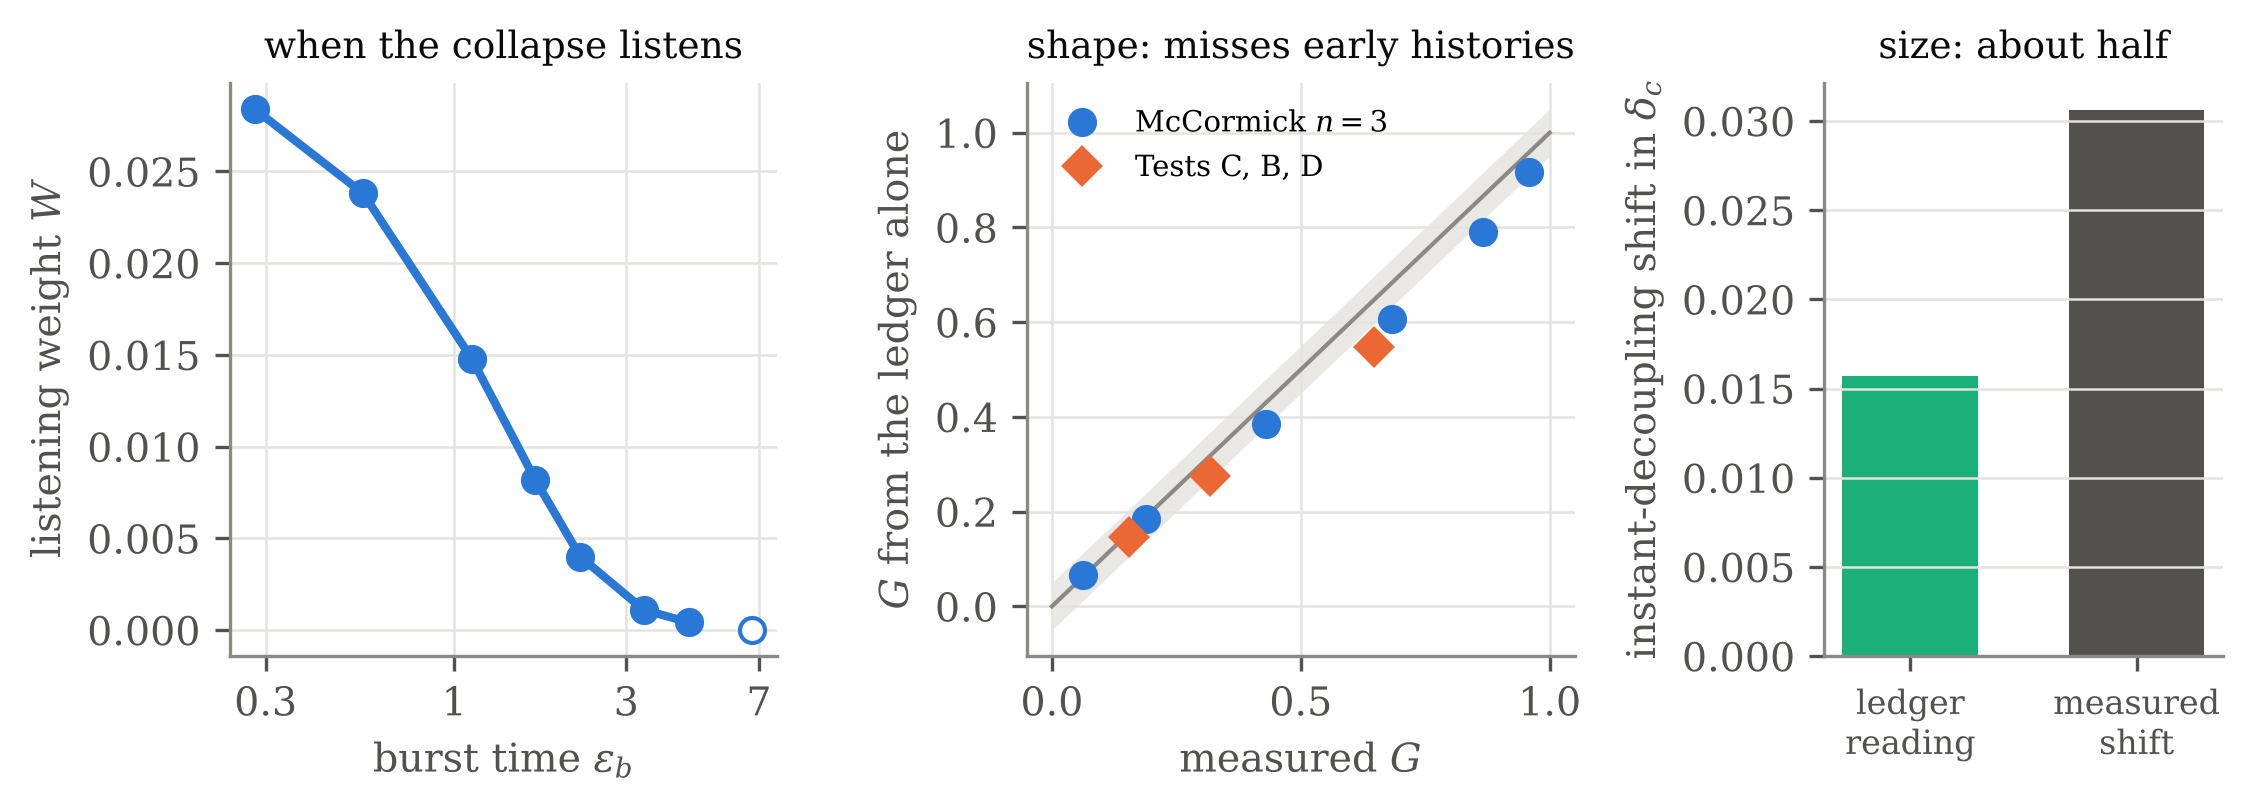
\includegraphics[width=\textwidth]{figs/jfig4_ledger.png}
\caption{The ledger test. Left: the measured listening weight, the threshold shift per unit of ledger written by a burst of free streaming at $\epsilon_b$ (open point: no effect at $\epsilon_b=6$). Centre: $G$ predicted from the ledger alone against the measured value, with the pre-registered kill band $\pm0.05$; the early histories fall outside it. Right: the ledger reads about half of the instantaneous-decoupling shift.}\label{fig:ledger}\end{figure}

\section{Limits and open steps}

\begin{itemize}
\item The finite theorems stand on their stated hypotheses. The identifications of the rungs with memory, light, time and budget are readings of standard quantities \grade{H}; Proposition~\ref{prop:ladder} is classical.
\item Proposition~\ref{prop:edge} is proved for one chart. Whether a sign wall of an analytic idempotent family always sits on its self-adjoint locus is untested.
\item Nothing here derives a gravitational field equation, an area law or a spacetime metric. The sign wall is a wall of a parameter form, not a horizon \cite{GLO}.
\item The neutrino runs use McCormick's relaxation-time collision term, spherical symmetry and a Gaussian profile. The ledger test used a fully coupled base at $\kappa/H=10^4$, not the cap, and its coupling bursts were ramped over ten steps because a direct switch crashes the code. K5 rests on one approximately matched pair.
\item The Lean coverage is finite and named per statement; analytic, contour and variational steps are written proofs.
\end{itemize}

\section{Summary}

The present must keep whatever its reading does not close over, and the cost of moving what it keeps is one number, the weight between. That number, read at four powers of the gap, is memory geometry, light's response, the energy variance and the oscillator budget, tied by one convexity. A record written across a cut moves no faster than twice the square root of the weight times the cut's sensitivity. The kept subspace sees neither a scale nor a constant; a clock sees constants as differences; the contour ledger sees them directly. When the tangent form changes sign, the ledger passes through, the wall sits where the projector becomes orthogonal, and a probe sees it only when read with its phase. Neutrinos leaving a collapsing patch obey the same speed limit, remember how they left, and keep half of that memory in the light that has gone and half in the light still going.

\begin{thebibliography}{99}
\bibitem{WB} J.~Beasley, \emph{The Weight Between: what the present must keep, and what it costs to move it}, v1.1 (26 October 2026).
\bibitem{OSL} J.~Beasley, \emph{The Offset Speed Limit: rate is weight}, v1.1 (26 October 2026).
\bibitem{LKL} J.~Beasley, \emph{Light Keeps the Ledger: Matter, Direction, and the Wall Between Them}, research edition 7.2, Zenodo, doi:10.5281/zenodo.23043570 (2026).
\bibitem{GLO} J.~Beasley, \emph{The Ledger Outlives the Metric}, full research edition 6, Zenodo, doi:10.5281/zenodo.22959910 (2026).
\bibitem{NL} J.~Beasley, \emph{When the Neutrinos Leave: Decoupling History and the Threshold for Primordial Black Hole Formation}, v3.1 (31 October 2026); Lean statements at github.com/dicipler-pixel/neutrinos-leave-lean.
\bibitem{CE} J.~Beasley, \emph{Non-Normality Is Connection Energy}, Zenodo, doi:10.5281/zenodo.22804072 (2026).
\bibitem{OBB} J.~Beasley, \emph{The Offset Belongs to the Boundary}, v31, Zenodo, doi:10.5281/zenodo.22555919 (2026).
\bibitem{McC} S.~McCormick, \emph{Free-streaming neutrinos raise the threshold for primordial black hole formation}, preprint (2026); data and scripts doi:10.5281/zenodo.23808375.
\bibitem{McCcode} S.~McCormick, PBH\_neutrino\_simulation, github.com/quasilocal/PBH\_neutrino\_simulation (2026).
\bibitem{Kalman} R.~E.~Kalman, On the general theory of control systems, Proc.\ First IFAC Congress (1960).
\bibitem{Zwanzig} R.~Zwanzig, Memory effects in irreversible thermodynamics, Phys.\ Rev.\ 124, 983 (1961).
\bibitem{AA} J.~Anandan and Y.~Aharonov, Geometry of quantum evolution, Phys.\ Rev.\ Lett.\ 65, 1697 (1990).
\bibitem{MT} L.~Mandelstam and I.~Tamm, The uncertainty relation between energy and time in non-relativistic quantum mechanics, J.\ Phys.\ USSR 9, 249 (1945).
\bibitem{HLP} G.~H.~Hardy, J.~E.~Littlewood and G.~P\'olya, \emph{Inequalities}, Cambridge University Press (1952).
\bibitem{BL} S.~M.~Barnett and R.~Loudon, Optical Thomas--Reiche--Kuhn sum rules, Phys.\ Rev.\ Lett.\ 108, 013601 (2012).
\bibitem{SWM} I.~Souza, T.~Wilkens and R.~M.~Martin, Polarization and localization in insulators: generating function approach, Phys.\ Rev.\ B 62, 1666 (2000).
\bibitem{OF} Y.~Onishi and L.~Fu, Quantum weight: a fundamental property of quantum many-body systems, arXiv:2406.06783 (2024).
\bibitem{Pant} A.~Pantsialei, Harmonic rigidity at fixed spectral gap in one dimension, arXiv:2512.24790 (2025).
\bibitem{COW} R.~Colella, A.~W.~Overhauser and S.~A.~Werner, Observation of gravitationally induced quantum interference, Phys.\ Rev.\ Lett.\ 34, 1472 (1975).
\end{thebibliography}

\appendix
\sloppy
\section{Proofs}

\paragraph{A.1 Theorems~\ref{thm:early}--\ref{thm:close}.} Let $p$ be the minimal polynomial of $L$, degree $d\le\dim V$. Dividing $x^n$ by $p$ writes every $L^n$ as a combination of $I,\dots,L^{d-1}$, so $RL^k\delta=0$ for $k<d$ gives $RL^n\delta=0$ for all $n$. If $\delta\in N_\infty$ then $RL^n(L\delta)=RL^{n+1}\delta=0$, so $L\delta\in N_\infty$, and $n=0$ gives $N_\infty\subseteq\ker R$. For Theorem~\ref{thm:least}: if $F\delta=0$ then $F(v+\delta)=Fv$, so every future reading of $\delta$ vanishes and $\delta\in N_\infty$; $F$ then factors through $V/\ker F\twoheadrightarrow V/N_\infty$. For Theorem~\ref{thm:close}: if $RL=AR$, $Rv=0$ gives $RLv=0$; conversely, if $\ker R\subseteq\ker RL$, $RL$ factors through $R$, i.e.\ $RL=AR$; induction gives $\ker R\subseteq\ker RL^n$, so $N_\infty=\ker R$. $\square$

\paragraph{A.2 Equations~\eqref{eq:kernel}--\eqref{eq:EB}.} Variation of constants on $\dot y=-iH_{QQ}y-iB^\dagger x$ gives $y(t)=e^{-iH_{QQ}t}y(0)-i\int_0^te^{-iH_{QQ}(t-s)}B^\dagger x(s)ds$; substituting into $\dot x$ gives \eqref{eq:kernel}. At $u=0$, $\Tr K(0)=\Tr BB^\dagger=\F{B}^2$. $\square$

\paragraph{A.3 Proposition~\ref{prop:offdiag} and \eqref{eq:gEB}.} Multiply $V=PV+VP$ by $P$ on both sides: $PVP=2PVP$, so $PVP=0$; likewise $(1-P)V(1-P)=0$, and expanding $V=(P+1-P)V(P+1-P)$ leaves the two cross blocks. With $B=PH(1-P)$, $[H,P]=(1-P)HP-PH(1-P)=B^\dagger-B$ with the two terms in opposite blocks, so $\F{[H,P]}^2=2\F{B}^2$. For $P=|\psi\rangle\langle\psi|$, $\F{B}^2=\langle\psi|H(1-P)H|\psi\rangle=\langle H^2\rangle-\langle H\rangle^2$. For orthogonal $P$ and Hermitian tangents $V,W$, $Q(V,W)=\Tr(X_V^\dagger X_W)$ with $X_V=(1-P)VP$ is a Gram form; for two real directions $\det$ of the $2\times2$ Hermitian matrix $Q$ is $\det g-\Omega^2/4\ge0$. $\square$

\paragraph{A.4 Propositions~\ref{prop:ladder}, \ref{prop:rung1} and Corollary~\ref{cor:alpha}.} For $a<b<c$ put $\theta=(c-b)/(c-a)$, so $b=\theta a+(1-\theta)c$. H\"older's inequality with exponents $1/\theta$ and $1/(1-\theta)$ on $\sum|K|^2|\Delta|^b=\sum(|K|^{2\theta}|\Delta|^{\theta a})(|K|^{2(1-\theta)}|\Delta|^{(1-\theta)c})$ gives $S_b\le S_a^\theta S_c^{1-\theta}$, with equality iff $|\Delta|$ is constant on the support. For the ground row: perturbing the ground state of $H=\operatorname{diag}(d)$ by $K$ gives $\langle n|\partial0\rangle=K_{n0}/(d_0-d_n)$, so the fidelity metric is $\sum_n|K_{n0}|^2/\Delta_n^2=S_{-2}$; the static response is $\alpha_0=2\sum_n|K_{n0}|^2/\Delta_n=2S_{-1}$; $\Var_0K=\sum_{n\ne0}|K_{n0}|^2=S_0$. Since $[H,K]_{mn}=(d_m-d_n)K_{mn}$, $[K,[H,K]]_{00}=\sum_n\big(K_{0n}(d_n-d_0)K_{n0}-(d_0-d_n)K_{0n}K_{n0}\big)=2\sum_n\Delta_n|K_{n0}|^2$. For $K=qx$, $H=p^2/2m+V$: $[H,x]=-i\hbar p/m$, $[x,[H,x]]=\hbar^2/m$, giving $q^2\hbar^2/2m$. With $(a,b,c)=(-2,-1,1)$, $\theta=2/3$: $S_{-1}\le S_{-2}^{2/3}S_1^{1/3}$, i.e.\ $\alpha_0\le2(g_{KK}^2F)^{1/3}$, with equality iff one $\Delta_n$ carries all the weight. $\square$

\paragraph{A.5 Theorem~\ref{thm:osl} and Corollary~\ref{cor:record}.} Since $C$ and $I-C$ commute and $\frac d{dt}\Tr f(C)=\Tr(f'(C)\dot C)$, $\dot\tau=-\Tr[((I-C)^{-1}+C^{-1})\dot C]=\Tr(W\dot C)$ with $W=-(C(I-C))^{-1}$. Lifting, $\dot\tau=\Tr(EWE^\dagger\dot P)=\Tr(F\dot P)$. By Proposition~\ref{prop:offdiag} only the off-diagonal part $T=PF(1-P)+(1-P)FP=[P,[P,F]]$ contributes. Cauchy--Schwarz for $\operatorname{Re}\Tr(XY)$ on Hermitian matrices gives $\dot\tau^2\le\F{T}^2\F{\dot P}^2=2g\F{T}^2$. Finally $\F{T}^2=2\Tr(PF^2-PFPF)=2\Tr(CW^2-CWCW)=2\Tr(W^2C(I-C))=-2\Tr W=2S$, using $[W,C]=0$. Equality in Cauchy--Schwarz is $\dot P=\lambda T$; since $T$ is off-diagonal, $[P,[P,T]]=T$ and $H=i\lambda[T,P]$ generates it. The corollary inserts $g=E_B$ from \eqref{eq:gEB}. For the $2\times2$ gap: idempotence gives $|b|^2=c(1-c)$ and $2\operatorname{Re}\bar b\dot b=\dot c(1-2c)$; with $g=\dot c^2+|\dot b|^2$, $S=1/(c(1-c))$, $\dot\tau=-\dot c/(c(1-c))$, the numerator of $4gS-\dot\tau^2$ is $4\dot c^2c(1-c)+\dot c^2(1-2c)^2-\dot c^2+4(\operatorname{Im}\bar b\dot b)^2=4(\operatorname{Im}\bar b\dot b)^2$. $\square$

\paragraph{A.6 Proposition~\ref{prop:readers}.} (a) $sH+cI$ has the eigenvectors of $H$ and the same ordering for $s>0$, so its spectral projectors, and every quantity built from them and their derivatives, are unchanged; a parameter-dependent $c(\lambda)I$ contributes tangent entries $\langle a|c'I|b\rangle=0$ for $a\ne b$. (b) $e^{-i(H+c)t}=e^{-ict}e^{-iHt}$; the phase cancels in $\langle\psi(t)|O|\psi(t)\rangle$ and survives as $e^{-i(c_1-c_2)t}$ in an overlap of two branches. (c) Holomorphic functional calculus on the selected cluster gives $Z_\Gamma(K)=\sum_j\log\lambda_j$; the eigenvalues of $K+cI$ are $\lambda_j+c$ and those of $\alpha K$ are $\alpha\lambda_j$, with the same Riesz projector. $\square$

\paragraph{A.7 Theorems~\ref{thm:neutral} and \ref{thm:cap}.} An idempotent is similar to $\operatorname{diag}(I_k,0)$; trace is similarity-invariant, and a tangent is $D=\begin{pmatrix}0&X\\Y&0\end{pmatrix}$ with $X\in M_{k,n-k}$, $Y\in M_{n-k,k}$ independent, so $q(D)=\operatorname{Re}\Tr(XY)$. With $U=(X+Y^\dagger)/2$, $V=(X-Y^\dagger)/2$, $q=\F{U}^2-\F{V}^2$, each of $U,V$ having $2k(n-k)$ real coordinates. For Theorem~\ref{thm:cap}: differentiating $P^2=P$ twice gives $PD+DP=D$ and $PE+EP+2D^2=E$ with $E=P''(0)$; constant rank gives $\Tr D=\Tr E=0$, so $\Tr(PD)=0$ and $\Tr(PE)=-\Tr D^2$; Taylor expansion then gives the overlap formula, and if $q(D)<0$ the remainder is dominated for small $t$. $\square$

\paragraph{A.8 Theorem~\ref{thm:chart} and Proposition~\ref{prop:edge}.} Write $u=(1,z)^\top$, $v=(1,w)^\top$; then $P=uv^\top/(v^\top u)$ with $v^\top u=1+zw\ne0$ on the box since $|zw|<1$, so $P^2=P$ and $\Tr P=1$. At $x=0$, $1+zw=1-y^3$, and exact evaluation of $\tfrac12\operatorname{Re}\Tr(\partial_iP\,\partial_jP)$ gives $g_{xx}=(1-y^3)^{-2}$, $g_{xy}=0$, $g_{yy}=-2y(1-y^3)^{-2}$. Since $HP=(2+y/10)P$ and $H(I-P)=(5+y/5)(I-P)$, the eigenvalues are $2+y/10$ and $5+y/5$, separated by $3+y/10$; the circle $|z-2|=0.4$ encloses only the first, and functional calculus gives $N=1$, $Z=\log(2+y/10)$. (i) A rank-one idempotent $uv^\top/(v^\top u)$ is self-adjoint iff its range and co-range coincide, i.e.\ $v\propto\bar u$: $(1,w)\propto(1,\bar z)$, so $w=\bar z$, i.e.\ $x+iy^2=x-iy$, i.e.\ $y^2=-y$, whose only root in the box is $y=0$. (iii) $\partial_zP=r\,v^\top/(1+zw)$ with $r=e_2-wu/(1+zw)$, and $v^\top r=w-w(1+zw)/(1+zw)=0$, so $(\partial_zP)^2=(v^\top r)\,r\,v^\top/(1+zw)^2=0$. On $y=0$, $\partial_yz=i$ and $\partial_yw=2iy=0$, so $\partial_yP=i\,\partial_zP$, a nonzero rank-one nilpotent ($r\ne0$), hence not self-adjoint (a self-adjoint nilpotent is zero). Then $\operatorname{Re}\Tr(\partial_yP)^2=0$ while $\F{\partial_yP}^2>0$. (ii) On $y=0$, $P=(1+x^2)^{-1}\begin{pmatrix}1&x\\x&x^2\end{pmatrix}$ is real and $\partial_xP$ is real symmetric with $\tfrac12\Tr(\partial_xP)^2=(1+x^2)^{-2}$; $g_{yy}=0$ by (iii), and $g_{xy}=\tfrac12\operatorname{Re}\Tr(\partial_xP\,i\partial_zP)=0$ by symbolic evaluation. So $\det g=0$ on the line. Over the whole box exact factorisation gives $\det g=-y\,\mathcal A\,\mathcal B/\mathcal D^4$ with $\mathcal A=x^4+2x^2y^5+4x^2y^4+2x^2+y^6-2y^3+1$, $\mathcal B=2x^4-3x^2y^3+2x^2y^2+x^2y+4x^2+2y^6-4y^3+2$ and $\mathcal D=(1-y^3)^2+x^2(x^2+y^4+y^2+2)>0$. With $|x|,|y|<\tfrac14$, $\mathcal A\ge1-2|y|^3-2x^2|y|^5>0.96$ and $\mathcal B\ge2-4|y|^3-3x^2|y|^3-x^2|y|>1.9$, so $\det g$ has the sign of $-y$ for every $x$: positive below the line, negative above. $\square$

\paragraph{A.9 Theorem~\ref{thm:source}.} With $R(z)=(z-K)^{-1}$ and $\frac d{dt}R=RBR$, $\partial_tZ=\frac1{2\pi i}\oint\log z\,\Tr(RBR)\,dz=-\frac1{2\pi i}\oint\log z\,\partial_z\Tr(BR)\,dz$. Integrating by parts on the closed contour gives $\frac1{2\pi i}\oint z^{-1}\Tr(BR)\,dz=\Tr(BP_\Gamma K^{-1})$ by functional calculus, $z^{-1}$ being analytic inside $\Gamma$. For $K=K^\dagger>0$, $P_\Gamma K^{-1}=\sum_{\lambda\in\Gamma}\lambda^{-1}P_\lambda\ge0$ with range $\operatorname{Ran}P_\Gamma$. Polarisation: $q(e_i+e_j)-q(e_i)-q(e_j)=2\operatorname{Re}A_{ij}$ and $q(e_i+ie_j)-q(e_i)-q(e_j)=-2\operatorname{Im}A_{ij}$ for Hermitian $A$; for general $A$ the complex readings give $A_{ij}+A_{ji}$ and $A_{ij}-A_{ji}$ separately, while their real parts give only $\tfrac12(A+A^\dagger)$, which is Proposition~\ref{prop:readout}(b). $\square$

\paragraph{A.10 Equations~\eqref{eq:nukernel} and \eqref{eq:nuspeed}.} On the hidden block the collision term is $\sigma(\epsilon)I$, which commutes with $M_{QQ}$, so the propagator factorises as stated; variation of constants and $\langle0|M=c_0\langle1|$ give \eqref{eq:nukernel}. With $D=-\sigma(I-P_0)\le0$, $\frac d{d\epsilon}\lVert v\rVert^2=-2\sigma\lVert(I-P_0)v\rVert^2\le0$; $\dot v_0=-ikc_0v_1$, so $|\dot A|\le2kc_0|v_0||v_1|\le2\sqrt{E_B}\sqrt{A(1-A)}$. $\square$

\section{Computational record}

The computations listed here were run with their kill conditions written in the script header before the run; the symbolic checks of Propositions~\ref{prop:edge} and \ref{prop:rung1} are exact. Scripts, outputs and logs are in the supplementary archive.

\begin{center}\small\begin{tabular}{p{4.6cm}p{6.6cm}p{3.6cm}}\toprule
script & what it checks & outcome\\\midrule
WEIGHT-BETWEEN-CORE-01 & \eqref{eq:gEB}, Theorem~\ref{thm:osl}, ladder, connection energy & all pass~\cite{WB,OSL}\\
C4-RICHARDSON-01 & equality case of Theorem~\ref{thm:osl} & $7\times10^{-9}$\\
WEIGHT-CONSTANT-01, WEIGHT-SCALE-SIGN-01 & Proposition~\ref{prop:readers}(a),(b) & pass\\
JOIN\_CHECKS\_01 & Propositions~\ref{prop:rung1}, \ref{prop:readers}(c), Cor.~\ref{cor:alpha}, \eqref{eq:nuspeed} & all four pass\\
GRAV\_RETEST\_01 & 18 finite claims of~\cite{GLO}, among them Theorems~\ref{thm:neutral}, \ref{thm:cap}, \ref{thm:chart}, \ref{thm:source} & 16 pass; 2 differ from printed values only in the last digit\\
SOURCE\_WALL\_01 & Propositions~\ref{prop:edge} (grid), \ref{prop:readout} & all lines met\\
symbolic (SymPy) & Proposition~\ref{prop:edge}, the factorisation of $\det g$ & exact\\
Neutrinos.Memory (Lean) & Props~\ref{prop:edge}(i),(iii), the one-mode gap and \eqref{eq:onemode}, the middle ladder rung, \ref{prop:readers}(c) & CI: 84 theorems, standard axioms, 11 false controls rejected\\
JOINT-FIGURES-01 & Figures~\ref{fig:ladder}--\ref{fig:ledger} & computed\\
run\_nuc\_n3, trisect3 & Tests A--D and controls & as tabulated~\cite{NL}\\
witness\_run, witness\_kernel & matched-pair witness & every call as predicted\\
run\_burst, ledger, predict & ledger test, K1--K5 & K2 fails; others pass\\\bottomrule
\end{tabular}\end{center}

\end{document}
